
\section{Estimation}

\begin{transitionframe}

    \rmfamily % Font
    
    \begin{center}
    {\Huge \textbf{\textcolor{white}{Estimation}}}
    \end{center}
  
\end{transitionframe}

\begin{frame}

    \frametitle{Empirical model} % Title
    \framesubtitle{}  % Subtitle
    \rmfamily % Font
    
    \begin{wideitemize}
        \item Individual-level event study for different minimum wage quantiles: \textcolor{fgre}{Arkhangelsky, Kazuharu and, Zohar (in progress)}
    \end{wideitemize}
    
    \begin{equation*}
        u_{it} = \alpha_i + \lambda_t + \sum_{k\geq h}\tau_{ik} + \beta X_{it} + \nu_{it}
    \end{equation*}
    with 
    \vspace{9pt}
    \begin{wideitemize}
        \item[\textcolor{fblu}{\textbullet}] \(\textcolor{fblu}{i}\): county, \(\textcolor{fblu}{t}\): time (year-month), \(\textcolor{fblu}{k = t - z_i}\): time difference from PDMP implementation year in county \(\textcolor{fblu}{i}\), \(\textcolor{fblu}{z_i}\)
        \item[\textcolor{fblu}{\textbullet}] \(\textcolor{fblu}{u_{it}}\): unemployment rate, \(\textcolor{fblu}{X_{it}}\): demographic covariates, \(\textcolor{fblu}{\nu_{it}}\): idiosyncratic shock 
    \end{wideitemize}
    \vspace{9pt}
    State-level changes must be exogenous at the county level for \textcolor{fblu}{identification} and no anticipation up to \(\textcolor{fblu}{h}\) periods
    
\end{frame}

\begin{frame}

    \frametitle{Results} % Title
    \framesubtitle{}  % Subtitle
    \rmfamily % Font
    
    \begin{center}
        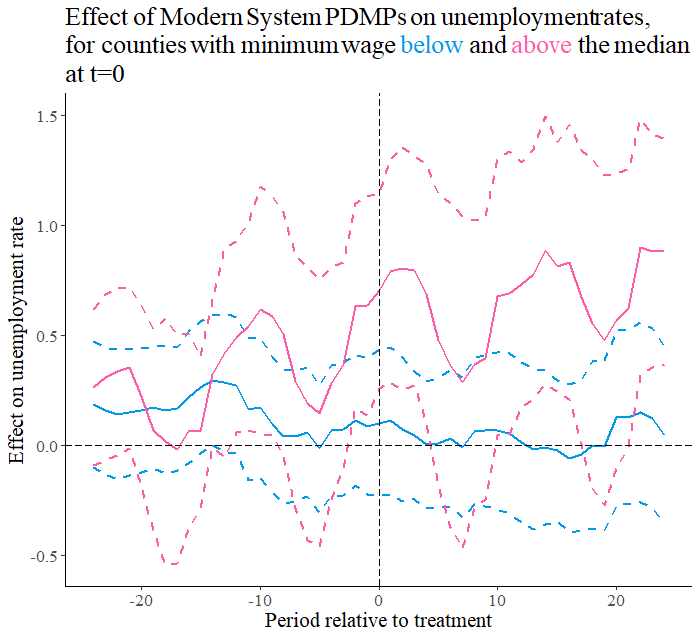
\includegraphics[scale=0.45]{mop_effects.png}
    \end{center}

\end{frame}


\begin{frame}

    \frametitle{Results} % Title
    \framesubtitle{}  % Subtitle
    \rmfamily % Font
    
    \begin{center}
        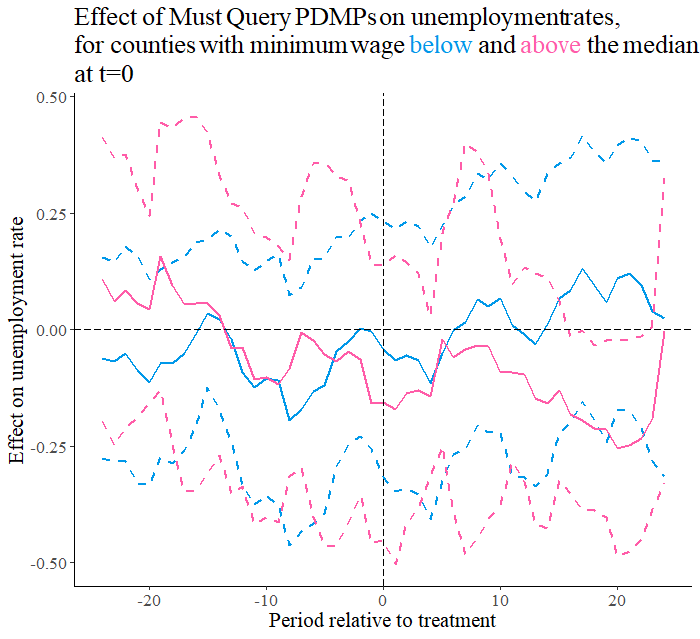
\includegraphics[scale=0.45]{pmq_effects.png}
    \end{center}

\end{frame}


\begin{frame}

    \frametitle{What is to be done?} % Title
    \framesubtitle{}  % Subtitle
    \rmfamily % Font
    
    \begin{wideitemize}
        \item Minimum wage measures of bindingness
        \vspace{9pt}
        \begin{wideitemize}
            \item Idea: we can estimate the effect of minimum wage on employment for wage bins
            \item Then assign, if significant, the coefficient to each county
            \item Sector compositions of the counties can also be relevant
        \end{wideitemize}
        \item I'm \textcolor{fblu}{open to suggestions}
        \item Participation rates might capture some of the effect
        \item Distribution of individual effects
    \end{wideitemize}
    
\end{frame}


